\documentclass[t]{beamer}

\usepackage{biblatex}
\usepackage{algorithm}
\usepackage{src/templates/algorithmicx/algpseudocode}

\setbeamerfont{footnote}{size=\tiny}

\input{header-presentation}
\title[FPGA for ENC!]{Investigating the Mapping of a Reconfigurable Cryptography Engine on a Zedboard}
\author[bobzhou@bu.edu]{by Boyou Zhou,\\Manuel Egele, Ajay Joshi}
\date[\today]{\today}

\begin{document}
\maketitle

\section*{FPGA for Encryption!}

\section{Intro: Why FPGA?}
\begin{frame}{What is ASIC, FPGA and GPP?}
    \begin{block}{ASIC}
        \begin{itemize}
            \item Application Specific Integrated Circuit
            \item Performance: Best, Cost: Highest, Time to Market: Slowest
        \end{itemize}
    \end{block}
    \begin{block}{FPGA}
        \begin{itemize}
            \item Field Programmable Gate Array
            \item Performance: Good, Cost: Normal, Time to Market: Normal 
        \end{itemize}
    \end{block}
    \begin{block}{GPP}
       \begin{itemize}
            \item General Purpose Processor
            \item Performance: Worst, Cost: Lowest, Time to Market: Fastest
       \end{itemize} 
    \end{block}
\end{frame}

\begin{frame}{Performance Comparison Between GPP, FPGA, and ASIC}
    \begin{figure}
        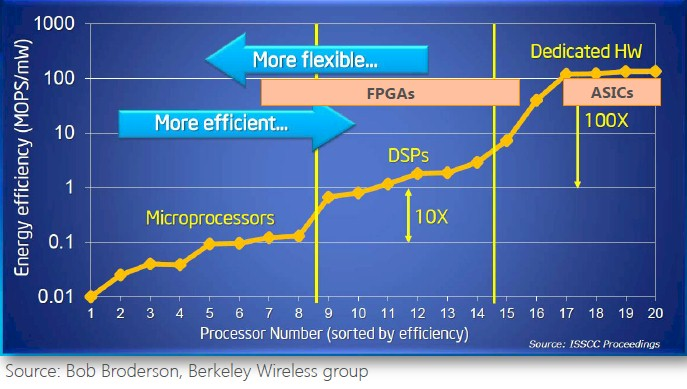
\includegraphics[width=3in]{img/microsoft-fpga-vs-cpu-vs-asic.png}
        \caption{FPGA, FPGA, and ASIC comparison from Microsoft\footcite{http://www.theplatform.net/2015/03/30/why-intel-might-buy-fpga-maker-altera}}
        \label{fig:performance-comparison}
    \end{figure}
\end{frame}

\begin{frame}{IoT Trend}
	\begin{figure}
        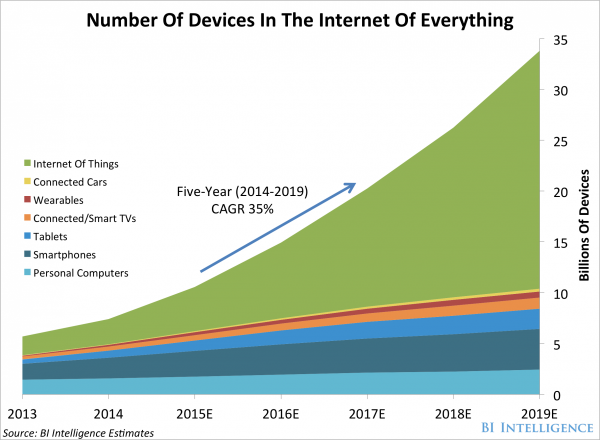
\includegraphics[width=2.5in]{img/iot_trend.png}
		\caption{Iot Trend\footcite{http://www.ironpaper.com/webintel/articles/internet-things-market-statistics-2015}}
		\label{fig:Iot_trend}
	\end{figure}
\end{frame}

\begin{frame}{Encryption Algorithm Upgrades}
	\begin{itemize}
		\item DES first published in 1977 and in Jan 1999, was publicly broken within 22 hours.
		\item AES first published in 1998 and was published as standard in 2002.\footcite{http://web.townsendsecurity.com/bid/72450/What-are-the-Differences-Between-DES-and-AES-Encryption}
		\item RC4 was invented in 1990. NSA moved from MD5 to SHA in 1993. Two years later, a weakness was found and switched to SHA1.
		\item In 2006, SHA1 was found not collision free. Now we use SHA256 mostly.\footcite{https://support.servertastic.com/deprecation-of-sha1-and-moving-to-sha2}
	\end{itemize}
\end{frame}

\begin{frame}{Main work}
	\begin{itemize}
		\item We propose reconfigurable crypto coprocessor for encryption upgrades.
		\item We synthesized and implemented AES, DES, SHA and RSA from Opencores to the Zedboard, and achieved run-time configuration.
		\item We compared our implementation with software implementation in terms of power, performance and EDP.
	\end{itemize}
\end{frame}

\begin{frame}{Related Works}
	\begin{itemize}
		\item Customized GPP: x86, ARM
		\item Crypto Coprocessor
		\item Crypto Processor 
		\item Crypto Arrays
	\end{itemize}
\end{frame}

\begin{frame}{FPGA-ENC-Implementation}
	\begin{figure}
        \includegraphics[width=1.5in]{img/customized_gpp.png}
        \includegraphics[width=1.5in]{img/crypto_coprocessor.png}\\
        \includegraphics[width=1.5in]{img/crypto_processor.png}
        \includegraphics[width=1.5in]{img/crypto_array.png}
		\caption{Basic Architecture and Memory Mapping\footnote{Architectures of flexible symmetric key crypto engines—a survey: From hardware coprocessor to multi-crypto-processor system on chip}}
		\label{fig:types_of_fpga_enc}
	\end{figure}
\end{frame}

\section{FPGA for Encryption}
\begin{frame}{Architecture}
	\begin{figure}
        \includegraphics[width=2in]{img/basic_arch.pdf}
        \includegraphics[width=2in]{img/mem_map.pdf}
		\caption{Basic Architecture and Memory Mapping}
		\label{fig:Iot_trend}
	\end{figure}
\end{frame}

\begin{frame}{Testbench Setup}
	\begin{itemize}
		\item Mapping DES, AES, SHA and RSA to Zedboard
		\item Evaluation on performance and power, compared to openssl implementation
		\begin{itemize}
			\item \tt Performance user level C code measurement
			\item \tt Power watts-up meter measurement
		\end{itemize}
		\item Run-time Configuration $\sim 90 msec$ 
		\begin{itemize}
			\item \tt bootgen generated separate bit files
		\end{itemize}
	\end{itemize}
\end{frame}

\section{Evaluation}
\begin{frame}{Utilization}
	\begin{table}[ht!]
		\begin{center}
			\begin{tabular}{c c c c c}
			   & AES & RSA & SHA & DES \\
			   \hline
			   Num of Gates & 41427     & 18687     & 29650     & 1275 \\
			   Utilization  & 77.87$\%$ & 35.11$\%$ & 55.71$\%$ & 2.4$\%$ 
			\end{tabular}
			\caption{Encryption Engine Utilization Summary on Zedboard}
			\label{table:gates}
		\end{center}
	\end{table}
\end{frame}

\begin{frame}{ENC Time}
	\begin{figure}
		\begin{center}
		\makebox[\textwidth][c]{\
		\includegraphics[width=1.5in]{img/aes-time.pdf}
		\includegraphics[width=1.5in]{img/rsa-time.pdf}}
		\makebox[\textwidth][c]{\
		\includegraphics[width=1.5in]{img/sha-time.pdf}
		\includegraphics[width=1.5in]{img/des-time.pdf}}
		\end{center}
		\caption{Time Comparison}
		\label{fig:time}
	\end{figure}
\end{frame}

\begin{frame}{ENC Power}
	\begin{figure}
		\begin{center}
		\makebox[\textwidth][c]{\
		\includegraphics[width=2.5in]{img/c-aes-pl-aes.pdf}
		\includegraphics[width=2.5in]{img/c-rsa-pl-rsa.pdf}}
		\end{center}
		\caption{Energy Comparison}
		\label{fig:power}
	\end{figure}
\end{frame}

\begin{frame}{ENC Power}
	\begin{figure}
		\begin{center}
		\makebox[\textwidth][c]{\
		\includegraphics[width=2.5in]{img/c-sha-pl-sha.pdf}
		\includegraphics[width=2.5in]{img/c-des-pl-des.pdf}}
		\end{center}
		\caption{Energy Comparison}
		\label{fig:power}
	\end{figure}
\end{frame}

\begin{frame}{ENC EDP}
	\begin{figure}
		\begin{center}
		\makebox[\textwidth][c]{\
		\includegraphics[width=1.5in]{img/aes-EDP.pdf}
		\includegraphics[width=1.5in]{img/rsa-EDP.pdf}}
		\makebox[\textwidth][c]{\
		\includegraphics[width=1.5in]{img/sha-EDP.pdf}
		\includegraphics[width=1.5in]{img/des-EDP.pdf}}
		\end{center}
		\caption{EDP Comparison}
		\label{fig:EDP}
	\end{figure}
\end{frame}

\section{Conclusion}
\begin{frame}{Conclusion}
    \begin{itemize}
        \item Performance Boost
        \item Energy Reduction
		\item Fast Configuration
    \end{itemize}
\end{frame}

\end{document}
